%%%%%%%%%%%%%%%%%%%%%%%%%%%%%%%%%%%%%%%%%%%%%%%%%%%%%%%%%%%%%%%%%%%%%%
% How to use writeLaTeX: 
%
% You edit the source code here on the left, and the preview on the
% right shows you the result within a few seconds.
%
% Bookmark this page and share the URL with your co-authors. They can
% edit at the same time!
%
% You can upload figures, bibliographies, custom classes and
% styles using the files menu.
%
% If you're new to LaTeX, the wikibook is a great place to start:
% http://en.wikibooks.org/wiki/LaTeX
%
%%%%%%%%%%%%%%%%%%%%%%%%%%%%%%%%%%%%%%%%%%%%%%%%%%%%%%%%%%%%%%%%%%%%%%
\documentclass{tufte-handout}

%\geometry{showframe}% for debugging purposes -- displays the margins

\usepackage{amsmath}

\usepackage{hyperref}
\hypersetup{
    colorlinks=true,
    linkcolor=blue,
    filecolor=magenta,      
    urlcolor=cyan,
}
\usepackage[super]{nth}

% Set up the images/graphics package
\usepackage{graphicx}
\setkeys{Gin}{width=\linewidth,totalheight=\textheight, keepaspectratio}
\graphicspath{{graphics/}}

\title{Week 2 :An Overview of Regression Methods }
\author[Ramzi Saouma}
%\date{24 January 2009}  % if the \date{} command is left out, the current date will be used

% The following package makes prettier tables.  We're all about the bling!
\usepackage{booktabs}

% The units package provides nice, non-stacked fractions and better spacing
% for units.
\usepackage{units}

% The fancyvrb package lets us customize the formatting of verbatim
% environments.  We use a slightly smaller font.
\usepackage{fancyvrb}
\fvset{fontsize=\normalsize}

% Small sections of multiple columns
\usepackage{multicol}
\usepackage{amsmath}
% Provides paragraphs of dummy text
\usepackage{lipsum}
\newcommand{\hlred}[1]{\textcolor{Maroon}{#1}}% prints in red
% These commands are used to pretty-print LaTeX commands
\newcommand{\doccmd}[1]{\texttt{\textbackslash#1}}% command name -- adds backslash automatically
\newcommand{\docopt}[1]{\ensuremath{\langle}\textrm{\textit{#1}}\ensuremath{\rangle}}% optional command argument
\newcommand{\docarg}[1]{\textrm{\textit{#1}}}% (required) command argument
\newenvironment{docspec}{\begin{quote}\noindent}{\end{quote}}% command specification environment
\newcommand{\docenv}[1]{\textsf{#1}}% environment name
\newcommand{\docpkg}[1]{\texttt{#1}}% package name
\newcommand{\doccls}[1]{\texttt{#1}}% document class name
\newcommand{\docclsopt}[1]{\texttt{#1}}% document class option name


\begin{document}

\maketitle% this prints the handout title, author, and date

\begin{abstract}
\noindent This week we cover the main and most commonly used regression models. Regression models fall under supervised learning and are applied to tasks where the target variable has a continuous value instead of a group of classes. We  start by refreshing our knowledge with a simple uni-variate linear regression and build our way up to end with Logistic regression.This week's material will be largely based on the book "Introduction to Statistical Learning"\cite{Tibshirani2017}. It is freely available here: \url{http://faculty.marshall.usc.edu/gareth-james/ISL/}. The book is a also a rich source of material for more in depth knowledge.
\end{abstract}

%\printclassoptions


\section{Outline: Learning 
Objectives}\label{sec:page-layout}

\begin{enumerate}
    \item \newthought{Linear Regression}
    \item \newthought{Multivariate Regression}
    \item \newthought{Ridge Regression}
    \item \newthought{Lasso Regression}
    \item \newthought{Polynomial Regression}
    \item \newthought{Logistic Regression}
\end{enumerate}
\subsection{Linear Regression}\label{sec:Regression}

\begin{figure}
  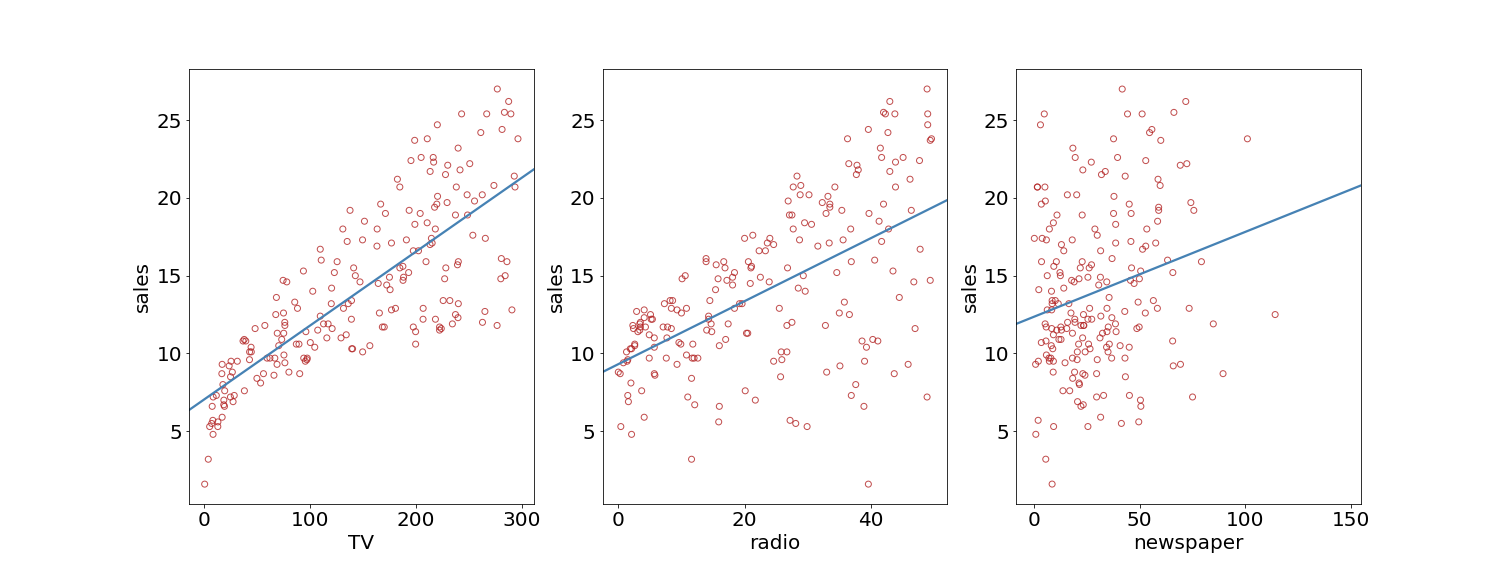
\includegraphics{Reg_1.png}
  \caption{Advertising Data. Can we predict future sales? is the relationship linear?.
  \emph{Linear Regression is a simple approach of supervised learning. It assumes that the relationship between the feature and the target is linear.}}
  \label{fig:textfig}
\end{figure}
 We assume that the linear regression model, which is a straight line, is mathematically expressed by the following equation\footnote{The betas are called coefficients or parameters. Epsilon is the error term, which is the difference between the predicted target given X and the observed y}:

\begin{equation}
    Y = \beta_0 + \beta_1X + \epsilon 
\end{equation}

The element that interest the most is the error term epsilon which could be written as below: 

\begin{equation}
    \epsilon_i =y_i - \hat{y}_i
\end{equation}
The errors also know as the residuals are the difference between the observed \( y_i \) and the estimated \( \hat{y_i}\) by our model\footnote{The superscript  \(\hat{}\)  denotes an estimated value. The superscript overline (-) denotes the sample mean of the underlying variable}. That is the grey distance in figure 2. 



\begin{figure}
  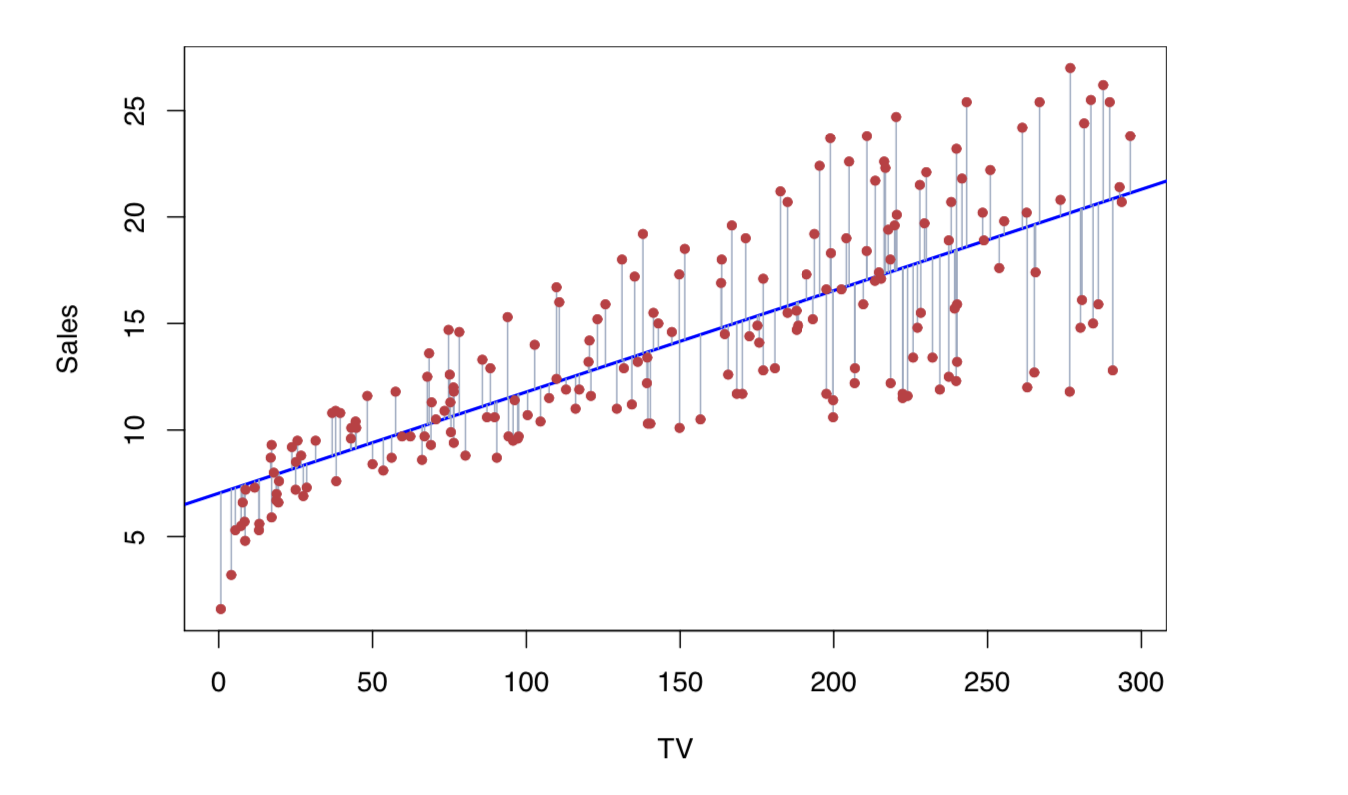
\includegraphics{Reg_2.png}
%  \checkparity This is an \pageparity\ page.%
  \caption{Based on the 
  \emph{Ordinary Least Squares model (OLS)}, the best fitting straight line is the ones that minimizes the error terms. In other word the one that minimizes the distance between the projected target and the observed target.}
  \label{fig:textfig}
  %\zsavepos{pos:textfig}
  \setfloatalignment{b}
\end{figure}

The simplest algorithm used to fit the straight line is Ordinary Least Squares (OLS). OLS estimates the betas by minimizing the below equation, also known as \hlred{residual sum of square}:
\begin{equation}
    RSS = \epsilon_1^2+\epsilon_2^2+...+\epsilon_n^2
\end{equation}

The minimizing values can be shown to be:
\begin{equation}
    \hat{\beta}_1 = \frac{\sum_{i=1}^{n}(x_i -\overline{x})(y_i -\overline{y})}{\sum_{i=1}^{n}(x_i -\overline{x})^2}
\end{equation}
\begin{equation}
    \hat{\beta}_0 = \overline{y}-\hat{\beta}_1\overline{x}
\end{equation}

\subsection{Assessing the Overall Accuracy of the Model}

\begin{figure}
  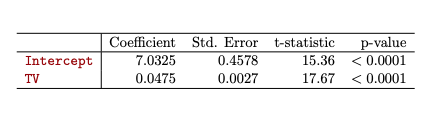
\includegraphics{reg_3.png}
%  \checkparity This is an \pageparity\ page.%
  \caption{
  \emph{Results for the advertising data}}
  \label{fig:textfig}
  %\zsavepos{pos:textfig}
  \setfloatalignment{b}
\end{figure}

\begin{equation}
    R^2 = \frac{TSS - RSS}{TSS},
\end{equation}
Where,
\begin{equation}
    TSS = \sum_{i=0}^{n}(y_i-\overline{y})^2,
\end{equation}

 The \hlred{\(R^2\)} is the most important indicator on how good the fit is. It is easy to show that the value of \hlred{\(R^2\)} falls between 0 and 1. As the residuals go to zero, \(R^2\) will converge to one. The closer it is to 1 the smaller are residuals the better is the fit. In machine learning and for the sake of this course we will use \(R^2\) as the main indicator of the quality of the model. 

\subsection{Multiple Linear Regression}

With a multi-dimentional regression the model becomes more complex:

\begin{equation}
    Y = \beta_0 + \beta_1X_1 +\beta_2X_2 + ... + \beta_pX_p + \epsilon
\end{equation}
In our particular marketing case we will be adding to new features, radio and newspaper adds, hoping we can learn more for a slightly more complex model. 
\begin{figure}
  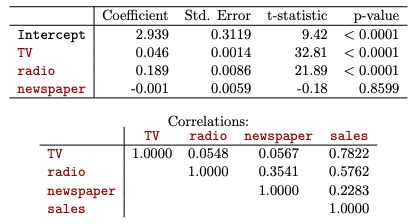
\includegraphics{reg5.png}
%  \checkparity This is an \pageparity\ page.%
  \caption{
  \emph{Results for the advertising data adding two new features Radio and Newspaper advertising}}
  \label{fig:textfig}
  %\zsavepos{pos:textfig}
  \setfloatalignment{b}
\end{figure}
While the math for estimating the parameters for a multiple regression gets more complicated, we are not concerned with that, given that python will do the work for us. In principle everything that applies to the one dimensional regression applies to the multiple regression model. In other world the \hlred{\(R^2\)} remains our most important indicator when it comes to the quality of model.
In an ideal world the \hlred{correlation} between different features is close to if not zero. With substantial correlation the variance of the parameters of each feature tend to increase, sometimes dramatically. Interpretations become hazardous since when one of the features changes everything else changes.  
 \begin{figure}
  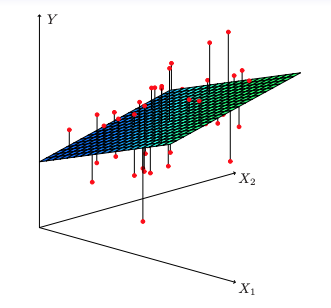
\includegraphics{reg_4.png}
%  \checkparity This is an \pageparity\ page.%
  \caption{
  \emph{In a two dimensional linear regression model we aim to fit a plane instead of a straight line}}
  \label{fig:textfig}
  %\zsavepos{pos:textfig}
  \setfloatalignment{b}
\end{figure}
\subsection{Deciding on the important features}

\begin{enumerate}
    \item \newthought{\hlred{All Subset Approach}}
    The most direct approach is called all subsets: we compute the OLS fit for all possible subsets of features and then choose between them based on some criterion that balances training error \hlred{\(R^2\)} with model size. 
    \item \newthought{\hlred{Forward Selection}}
    Begin with the null model — a model that contains an
intercept but no predictors. Fit p simple linear regressions and add to the null model
the variable that results in the lowest RSS. Add to that model the variable that results in the lowest
RSS amongst all two-variable models. Continue until some stopping rule is satisfied, for example
when all remaining variables have a p-value above some
threshold.
    
    \item \newthought{\hlred{Backward selection}}
    Start with all variables in the model. Remove the variable with the largest p-value — that is, the
variable that is the least statistically significant. The new (p − 1)-variable model is fit, and the variable with the largest p-value is removed. Continue until a stopping rule is reached. For instance, we may stop when all remaining variables have a significant p-value defined by some significance threshold.
    
\end{enumerate}

 \begin{figure}
  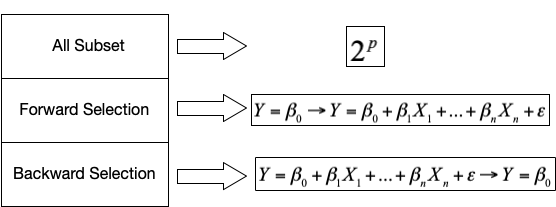
\includegraphics{multiple.png}
%  \checkparity This is an \pageparity\ page.%
  \caption{Selecting the optimal combination of features}
  \label{fig:textfig}
  %\zsavepos{pos:textfig}
  \setfloatalignment{b}
\end{figure}

\subsection{Ridge Regression}

As an alternative to the previous feature selection methodology, we can fit a model containing all p predictors using a technique that constrains or \hlred{regularizes}\footnote{In mathematics, statistics, and computer science, particularly in machine learning and inverse problems, regularization is the process of adding information in order to solve an ill-posed problem or to prevent overfitting.$source   :$ Wikipedia} the coefficient estimates, or equivalently, that shrinks the coefficient estimates towards zero. It may not be immediately obvious why such a constraint should improve the fit, but it turns out that shrinking the coefficient estimates can significantly reduce their variance.

\begin{marginfigure}%
  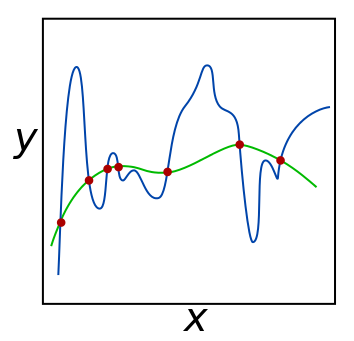
\includegraphics[width=\linewidth]{regulization.png}
  \caption{The green and blue functions both incur zero loss on the given data points. A learned model can be induced to prefer the green function, which may generalize better to more points drawn from the underlying unknown distribution, by adjusting lambda.$source:$ Wikipedia}
  \label{fig:marginfig}
\end{marginfigure}
Instead of minimizing the RSS as we did earlier, the ridge regression solve for the \(\hat{\beta}\) by minimizing the below equation:
\begin{equation}
    RSS + \lambda \sum_{j=1}^{p}\beta_j^2
   
\end{equation}
\\ The objective function we are minimizing is similar to the one we saw with simple regression but we are adding a new term \hlred{penalty term} where \(\lambda\) is a \emph{\hlred{tuning parameter}}\footnote{The ridge regression imposes constraint on the parameters betas. The tuning term \(\lambda\) regularizes the coefficients such that if the coefficients take large values the optimization function is penalized. As a result, we shrink the coefficients which helps to reduce the model complexity }.
\\As with least squares, ridge regression seeks coefficient estimates that fit the data well, by making the RSS small. However, the second term, \(\lambdada\) a shrinkage penalty, is small when \(\beta_1\), . . . , \(\beta_p \) are close to zero, and so it has the effect of shrinking the estimates of \(\beta_j \) towards zero. The tuning parameter \(\lambdada\) serves to control the relative impact of these two terms on the regression coefficient estimates. Selecting a good value for \(\lambdada\) is critical; cross-validation is used for this\footnote{We will look more into cross-validation techniques in \emph{Week 4} }.

\subsection{Scaling the Features}
\begin{enumerate}
    \item The standard least squares coefficient estimates are \hlred{scale equivariant}: multiplying \(X_j\) by a constant c simply leads to a scaling of the least squares coefficient estimates by a factor of 1/c. In other words, regardless of how the jth feature is scaled,\(X_j\hat{\beta_j}\) will remain the same.
    \item In contrast, the ridge regression coefficient estimates can change substantially when multiplying a given feature by a constant, due to the sum of squared coefficients term in the penalty part of the ridge regression objective function.
    \item Therefore, it is best to apply ridge regression after standardizing the predictors, using the formula
\end{enumerate}

\begin{equation}
    \Tilde{x}_i_j = \frac{x_{ij}}{\sqrt{\frac{1}{n}\sum_{i=1}^{n}(x_{ij}-\overline{x}_j)^2}}
\end{equation}
\subsection{Lasso Regression}
\\ Ridge regression does have one obvious disadvantage: unlike subset selection, which will generally select models that involve just a subset of the variables, ridge regression will include all p predictors in the final model.
\\ The Lasso is a relatively recent alternative to ridge regression that overcomes this disadvantage. The \hlred{lasso} coefficients \(\hat{\beta}_\lambda^L\), minimize the quantity:

\begin{equation}
    RSS +\lambda\sum_{j=1}^{p}|\beta_j|
\end{equation}
\begin{itemize}
    \item As with ridge regression, the lasso shrinks the coefficient
estimates towards zero.
    \item However, in the case of the lasso, the `1 penalty has the effect of forcing some of the coefficient estimates to be exactly equal to zero when the tuning parameter \(\lambda\) is sufficiently large.
    \item Similarly to the subset selection, the lasso performs \hlred{variable selection}.
    \item Lasso regression falls under the sparse models\footnote{\hlred{Sparse Models} are models where only a small fraction of parameters are non-zero – arise frequently in machine learning. Sparsity is beneficial in several ways: sparse models are more easily interpretable by humans, and sparsity can yield statistical benefits – such as reducing the number of examples that have to be observed to learn the model. In a sense, we can think of sparsity as an antidote to curse of dimensionality}, that is models that involve only a subset of the variables.
    \item similarly to the Ridge regression choosing for the right value of \(\lambda\) is key and it is achieved by doing cross-validations
\end{itemize}

\subsection{Polynomial Regression}


 \begin{figure}
  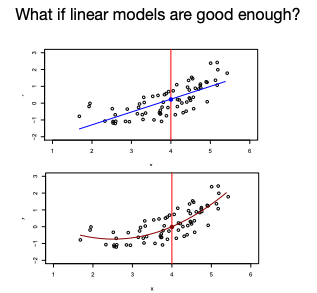
\includegraphics{polynomial.png}
%  \checkparity This is an \pageparity\ page.%
  \caption{linear Vs Non-linear fitting}
  \label{fig:textfig}
  %\zsavepos{pos:textfig}
  \setfloatalignment{b}
\end{figure}


This is how a degree-n polynomial regression model looks like:

\begin{equation}
    y_i = \beta_0+\beta_1x_i+\beta_2x_i^2+\beta_3x_i^3+...+\beta_d x_i^d+\epsilon_i
\end{equation}

Obviously, the formula 12 applies to one feature X, where we have created new variables \(X_1 =X,     X_2=X^2,..., X_n=X^n\). This could also be applied to multiple features regressions like the below example where we try to predict income by looking at two features: years of education as well as seniority.



 \begin{figure}
  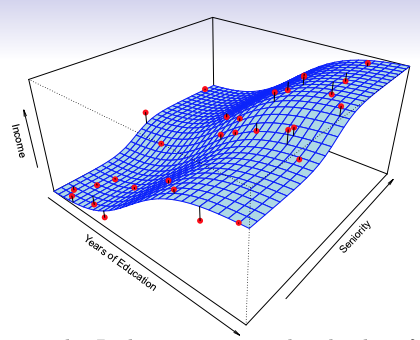
\includegraphics{poly_2.png}
%  \checkparity This is an \pageparity\ page.%
  \caption{2-dimentional non-linear regression}
  \label{fig:textfig}
  %\zsavepos{pos:textfig}
  \setfloatalignment{b}
\end{figure}


\subsection{Logistic Regression}

Even though, it falls under regression, most of the applications of logistic regressions are on classification problems, a topic that we will only cover next week. But assume that we solving for a task where the target variable takes a binary form. Like in the case we saw last week where we are trying to predict whether an email is spam or not based on some quantitative features. Or lets assume we are trying to predict whether a client is going to default on his credit card. The target variable in this case would be binary, default or no-default. 

  \begin{equation}
    Y=
    \begin{cases}
      0, & \text{if default} \\
      1, & \text{if no-default}
    \end{cases}
  \end{equation}


 \begin{figure}
  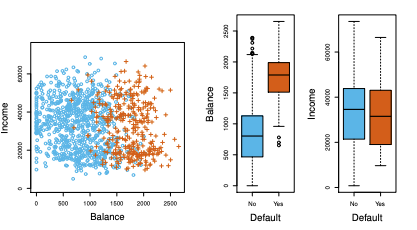
\includegraphics{logistic.png}
%  \checkparity This is an \pageparity\ page.%
  \caption{Credit Card Default based on income and balance. Default observations are denoted in orange.}
  \label{fig:textfig}
  %\zsavepos{pos:textfig}
  \setfloatalignment{b}
\end{figure}

Can we simply perform a \hlred{linear regression} of Y(default) on X(income and balance) and classify as Yes if Y >ˆ 0.5?

\begin{itemize}
    \item We probably could run a linear regression and the predicted value of Y could be interpreted as the probability of default. 
    \item The problem with linear regressions nothing is stopping \(\hat{Y}\) from getting values higher that one or negative.
\end{itemize}

Logistic regression uses the form:

\begin{equation}
    Y = \frac{e^{\beta_0+\beta_1X}}{{1+e^{\beta_0+\beta_1X}}}
\end{equation}
It is easy to see that as X goes to zero Y converge to zero and when X go to infinity Y converges to 1.

 \begin{figure}
  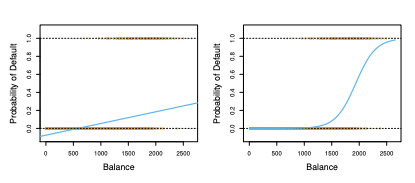
\includegraphics{log_1.png}
%  \checkparity This is an \pageparity\ page.%
  \caption{Logistic regression ensures that out estimate for Y lies between 0 and 1}
  \label{fig:textfig}
  %\zsavepos{pos:textfig}
  \setfloatalignment{b}
\end{figure}

Unlike the previous regressions, the logistic regression does not use ordinary least square method to solve for the parameters. Instead we use the \hlred{Maximum Likelihood Estimation}\footnote{In statistics, \hlred{maximum likelihood estimation (MLE)} is a method of estimating the parameters of a probability distribution by maximizing a likelihood function, so that under the assumed statistical model the observed data is most probable. $source$ Wikipedia} method which beyond the scope of this course.

\section{Learning Summary}

\begin{itemize}
    \item We have learned the concepts behind six different regression techniques
    \item We know how to interpret p-values, RSS and \(R^2\)
    \item we learned about different techniques to select the important features: subset, forward and backward selections
    \item We introduced the concept of regularization and the tuning parameter \(\lambda\)
    \item We introduced one scaling method for features
    \item We understand the advantage of sparse models
\end{itemize}

\bibliography{sample-handout}
\bibliographystyle{plainnat}



\end{document}